\section{Query Optimizer Integration}
\label{integration}

In the earlier sections, given a user query, the modified operator
implementations were used for the \emph{standard} plan choice
of the PostgreSQL optimizer. That is, while the execution engine was PCM-conscious,
the presence of PCM was completely \emph{opaque} to the optimizer.
However, given the read-write asymmetry of PCM in terms of both latency and wear
factor, it is possible that alternative plans, capable of providing better
performance profiles, may exist in the plan search space. To discover
such plans, the database query optimizer needs to incorporate PCM
awareness in both the operator cost models and the plan enumeration
algorithms.

Current query optimizers typically choose plans using a latency-based
costing mechanism. We revise these models to account for the additional
latency incurred during writes. Additionally, we introduce a new metric of
\emph{write cost} in the operator cost model, representing the incurred
writes for a plan in the PCM environment, using the estimators described in Sections~\ref{sort}
to \ref{gby}. We henceforth refer to the latency cost and the write cost
of a plan as {\bf LC} and {\bf WC}, respectively.

A new user-defined parameter, called the \emph{latency slack}, is
incorporated in the query optimizer.  This slack, denoted by $\lambda$,
represents the maximum relative slowdown, compared to the LC-optimal
query plan, that is acceptable to the user in lieu of getting better
write performance. Specifically, if the LC of the LC-optimal execution
plan $P_o$ is $C_o$ and the LC of an alternate plan $P_i$ is $C_i$, the
user is willing to accept $P_i$ as the final execution plan if $C_i \le
(1+\lambda) C_o$. The $P_i$ with the least WC satisfying this equation
is considered the WC-optimal plan.

With the new metric in place, we need to revise the plan enumeration
process during the planning phase. This is because the native optimizer
propagates only the LC-optimal (and interesting order) plans through
the internal nodes of the dynamic programming lattice, which may lead
to pruning of potential WC-optimal plans. On the other hand, propagating
the \emph{entire} list of sub-plans at each internal node can end up in
an exponential blow-up of the search space.  As an intermediate option between these
two extremes, we use a heuristic propagation mechanism at each internal
node, employing an algorithmic parameter, \emph{local threshold} $\lambda_l$
($\ge\lambda$). Specifically, let $p_i$ and $p_o$ be a generic sub-plan and the LC-optimal
sub-plan at a node, respectively, with $c_i$ and $c_o$ being their
corresponding LC values. Now, along with the LC-optimal and interesting
order sub-plans, we also propagate $p_i$ with the \emph{least} WC that
satisfies $c_i \le (1+\lambda_l) c_o$. We observed that
setting $\lambda_l = \lambda$ delivered reasonably good results in this respect.

\begin{figure}[htpb]
\centering
	
\subfloat[Performance of Alternative Plans]{
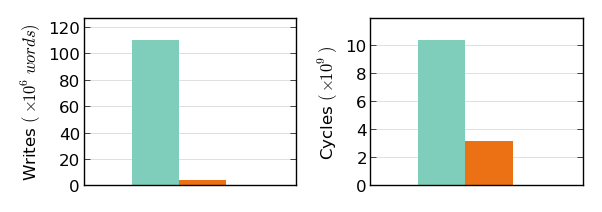
\includegraphics[height=29mm]{./fig/q13_alternate_plan.png}
}

\subfloat[Overall performance comparison]{
\begin{small}

  %\begin{tabular}{p{3cm}p{2cm}p{2cm}p{2cm}p{2cm}}
  \begin{tabular}{p{3.5cm}c c c c}
  \toprule                                                                                                
  
  \textbf{Metric} & \textbf{Opt(PCM-O)} & \textbf{Opt(PCM-O) } & \textbf{Opt(PCM-C)} & \textbf{Opt(PCM-C)}\\
  & \textbf{Exec(PCM-O) } & \textbf{Exec(PCM-C)} & \textbf{Exec(PCM-C)} & \textbf{Exec(PCM-O)}\\
  \midrule                                                                                                
  
  \textbf{Mega Word-Writes} &  $233.6$ & $110.6$ & $4.66$ & $12.8$\\ 
  \textbf{Giga Cycles} &  $13.1$ & $10.4$ & $3.2$ & $4.5$\\ 
  \bottomrule                                                                                             
  \end{tabular}                                                                                           
\end{small}                                                                                           
}
\caption{Integration with Query Optimization and Processing Engine}
\label{fig:perf_comp}
\end{figure}

In light of these modifications, let us revisit Query Q13, for which
the default plan was shown in Figure~\ref{fig:plan_trees}(a). With
just the revised latency costs (i.e. $\lambda$ = 0), the optimizer
identified a new execution plan wherein the merge left-join between
the \textit{customer} and \textit{orders} tables is replaced
by a hash left-join.  The relative performance of these two
alternatives with regard to PCM writes and CPU cycles are shown in
Figure~\ref{fig:perf_comp}(a). We observe here that there is a \emph{huge
difference} in both the query response times as well as write overheads
between the plans.  Specifically, the alternative plan reduces the writes
by well over an order of magnitude!  As we gradually increased the
latency slack value, initially there was no change in plans. However,
when the slack was made as large as 5, the hash left-join gave way to
a nested-loop left-join, clearly indicating that the nested-loop join
provides write savings only by incurring a steep increase in latency cost.


To put matters into perspective, Figure~\ref{fig:perf_comp}(b) summarizes
the relative performance benefits obtained as the database layers are
gradually made PCM-conscious (in the figure, the labels Opt and Exec
refer to Optimizer and Executor, respectively, while PCM-O and PCM-C
refer to PCM-Oblivious and PCM-Conscious, respectively). For the sake of
completeness, we have also added results for the case when the Optimizer
is PCM-C but the Executor is PCM-O (last column). The results clearly
indicate that future query optimizers for PCM-based architectures need
to incorporate PCM-Consciousness at \emph{both} the Optimizer and the
Executor levels in order to obtain the best query performance. 


